\scanpage{63}
% letterhead
\begin{tabular}{c}
UNIVERSITE DES SCIENCES ET TECHNIQUES\\
DU LANGUEDOC\\
---\\
INSTITUT DE MATHEMATIQUES\\
Place Eugène Bataillon\\
34060 MONTPELLIER CEDEX
\end{tabular}
\hfill Montpellier, le

\[
\begin{aligned}
&\deleted{(r_1+r_{i-1})+}\\
&(r_1\ldots+r_{i-1})+(r_2\ldots+r_{j-1})+(r_3+\ldots+r_{k-1})\\
&i\ge3 \qquad\qquad\qquad\unsure{{}+r_1}\\
&r_1+2(r_2\ldots+r_{i-1})
\end{aligned}
\]
\[
\begin{aligned}
&\delta_1\ -\ \delta_8\,\underline{\delta_9}
&&r_1&&r_1+2r_2&&i-1&&i{}+j+\unsure{h|k}-6\\
&\delta_1\ -\ \underline{\delta_n}\,\delta_{n+1}
&&r_1+r_2+r_3&& &&j-2\\
&n+1+9\le27&&r_2+r_3+r_4&& &&k-3\\
&n\le17&&r_3+r_4+r_5
\end{aligned}
\]
\figure{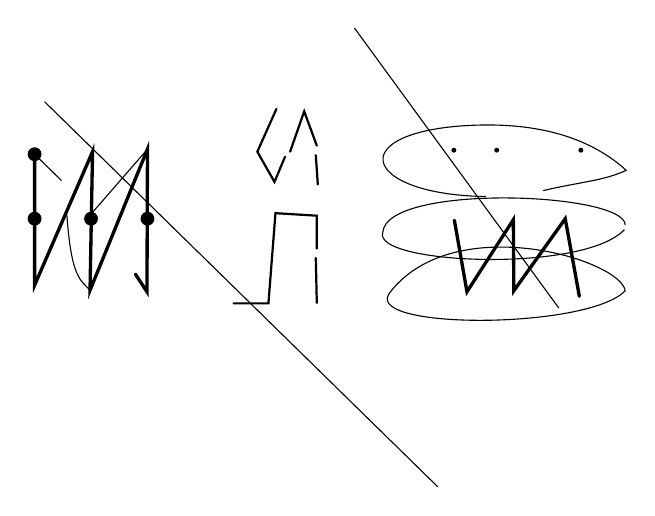
\begin{tikzpicture}[x=.64cm,y=.64cm,line cap=round]
\draw[very thick] (0,2.6)--(0,0)--(1.15,2.65)--(1.1,-.1)--(2.24,2.7)--(2.23,-.13)--(2.0,.22);
\draw (0,2.6)--(.53,2.08) (.64,1.4) .. controls (.73,.14) and (.91,.11) .. (1.1,-.1) (1.11,1.4)--(2.24,2.7);
\foreach \x in {0,1.12,2.24}{\fill (\x,1.32) circle(2.5pt);}
\fill (0,2.6) circle(2.5pt);
\draw[thick] (4.8,3.5)--(4.42,2.65)--(4.76,2.05)--(4.97,2.55) (5.07,2.65)--(5.35,3.45)--(5.6,2.77) (5.58,2.58)--(5.62,2.0);
\draw[thick] (3.95,-.36)--(4.64,-.36)--(4.78,1.43)--(5.60,1.38)--(5.6,.73) (5.58,.54)--(5.60,-.35);
\draw (8.95,1.76) .. controls (6.55,1.8) and (6.13,2.98) .. (8.45,3.16) .. controls (10.24,3.29) and (11.2,2.77) .. (11.74,2.28) .. controls (11.28,2.07) and (10.88,2.06) .. (10.1,1.88);
\draw (11.72,1.20) .. controls (11.69,1.85) and (6.98,2.02) .. (6.91,1.05) .. controls (6.68,.42) and (10.88,.23) .. (11.70,1.1);
\draw (11.72,-.11) .. controls (11.63,.51) and (8.35,1.49) .. (7.07,-.12) .. controls (6.37,-.89) and (10.97,-.89) .. (11.72,-.11);
\foreach \x in {8.32,9.17,10.84}{\fill (\x,2.68) circle(.9pt);}
\draw[very thick] (8.33,1.29)--(8.58,-.13)--(9.5,1.3)--(9.51,-.11)--(10.53,1.32)--(10.81,-.22);
\draw[thin] (.2,3.64)--(8,-4.0) (6.35,5.1)--(10.4,-.45);
\end{tikzpicture}}

% Lower part read with the sheet rotated through 180 degrees.
\[
\begin{aligned}
r_0&=2\eta-\zeta\\
r_1&=\zeta_1-\zeta_2\\
r_2&=\zeta_2-\zeta_3\\
r_3&=\zeta_3-\zeta_4\\
r_4&=\zeta_4-\zeta_5\ .\\
r_5&=\zeta_5-\zeta_6\\
\deleted{\unsure{r_6}}&=\\
r_6&=\eta-\zeta_1-\zeta_2-\zeta_3
\end{aligned}
\qquad
\left.\begin{aligned}
3(r_1+r_2+r_3)&=3(\zeta_1-\zeta_4)\\
2r_4&=\deleted{\unsure{3}}\zeta_4\deleted{\unsure{+}}-2\zeta_5\\
\unsure{2}r_5&=\deleted{\unsure{2}}\zeta_5-\zeta_6
\end{aligned}\right\}\quad3\zeta_1-\zeta_4-\zeta_5-\zeta_6
\]
\figure{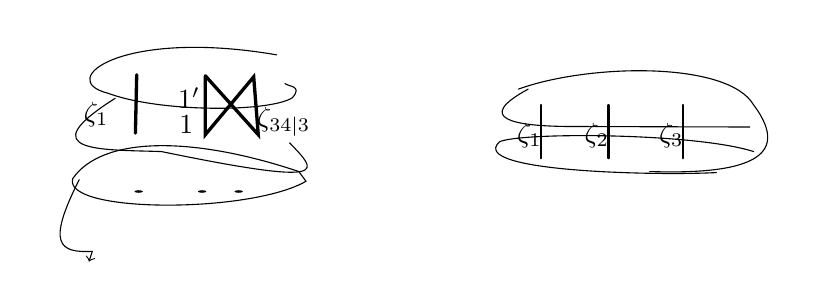
\begin{tikzpicture}[x=.83cm,y=.65cm,line cap=round]
\draw (2.8,2.7) .. controls (.43,3.22) and (-.6,2.21) .. (.22,1.95) .. controls (.99,1.58) and (2.67,1.57) .. (3.04,1.86) .. controls (3.21,2.1) and (2.97,2.08) .. (2.93,2.14);
\draw (.33,1.85) .. controls (-1.0,.78) and (.15,.85) .. (1.04,.81) .. controls (3.7,.11) and (3.42,.42) .. (3.0,.98);
\draw (3.14,.42) .. controls (1.48,1.13) and (.12,1.1) .. (-.32,.28) .. controls (-.47,-.4) and (2.40,-.4) .. (3.25,.23) --(3.14,.42);
\foreach \x in {.69,1.66,2.22}{\fill (\x,.03) ellipse(.065 and .025);}
\draw[very thick] (.66,2.31)--(.64,1.17) (1.71,2.29)--(1.71,1.14)--(2.45,2.27)--(2.52,1.14)--(1.71,2.29);
\node at (.04,1.53) {$\zeta_1$};\node at (1.46,1.85) {$\unsure{1'}$};\node at (1.42,1.33) {$\unsure{1}$};\node at (2.91,1.40) {$\zeta_{\unsure{34|3}}$};
\draw[->] (-.22,.26) .. controls (-.72,-1) and (-.53,-1.17) .. (-.02,-1.14)--(-.07,-1.34);
\draw (6.5,2.03) .. controls (7.58,2.53) and (9.71,2.58) .. (10.1,1.72) .. controls (10.72,.66) and (9.94,.36) .. (8.51,.42);
\draw (6.65,2.03) .. controls (5.81,1.45) and (6.43,1.31) .. (7.26,1.3)--(10.04,1.29);
\draw (10.10,.81) .. controls (9.2,1.18) and (6.51,1.19) .. (6.21,1.0) .. controls (5.70,.40) and (8.71,.34) .. (9.53,.40);
\foreach \x/\y in {6.85/1,7.88/2,9.02/3}{\draw[thick](\x,.68)--(\x,1.72);\node at (\x-.18,1.12) {$\zeta_{\y}$};}
\end{tikzpicture}}
% archive sheet number: 62
